\begingroup\sloppy
\section{Popis architektury systému}\label{sec:arch}

Systém je jedna aplikace v Javě rozdělená do tří vrstev. Prezentační vrstva obsahuje desktopovou aplikaci v JavaFX a webové rozhraní na vestavěném serveru \texttt{HttpServer} z JDK. Aplikační (business) vrstva obsahuje doménový model a aplikační služby. Datová vrstva ukládá data do databáze Oracle přes JDBC a soubory dokumentů do složky na disku. Vrstvy odpovídají balíčkům \texttt{cz.vsb.catering.presentation}, \texttt{cz.vsb.catering.business} a \texttt{cz.vsb.catering.data}. Třída \texttt{AppContext} načte konfiguraci, vytvoří datovou vrstvu a propojí služby. Obě uživatelská rozhraní dostávají služby pouze od ní. Oba diagramy v této kapitole jsou zakresleny podle UML~2.

\subsection{Diagram komponent}\label{sec:arch:komponenty}

Diagram komponent je kvůli čitelnosti rozdělen na dvě části. Obrázek~\ref{fig:komponenty} ukazuje prezentační a aplikační vrstvu s rozhraními aplikačních služeb. Obrázek~\ref{fig:komponenty-data} ukazuje rozhraní, která aplikační vrstva vyžaduje, a datovou vrstvu, která je implementuje. Poskytované rozhraní je zakresleno jako kulička, vyžadované rozhraní jako půlkruh. Přerušovaná šipka je závislost.

\clearpage
\begin{figure}[H]
  \centering
  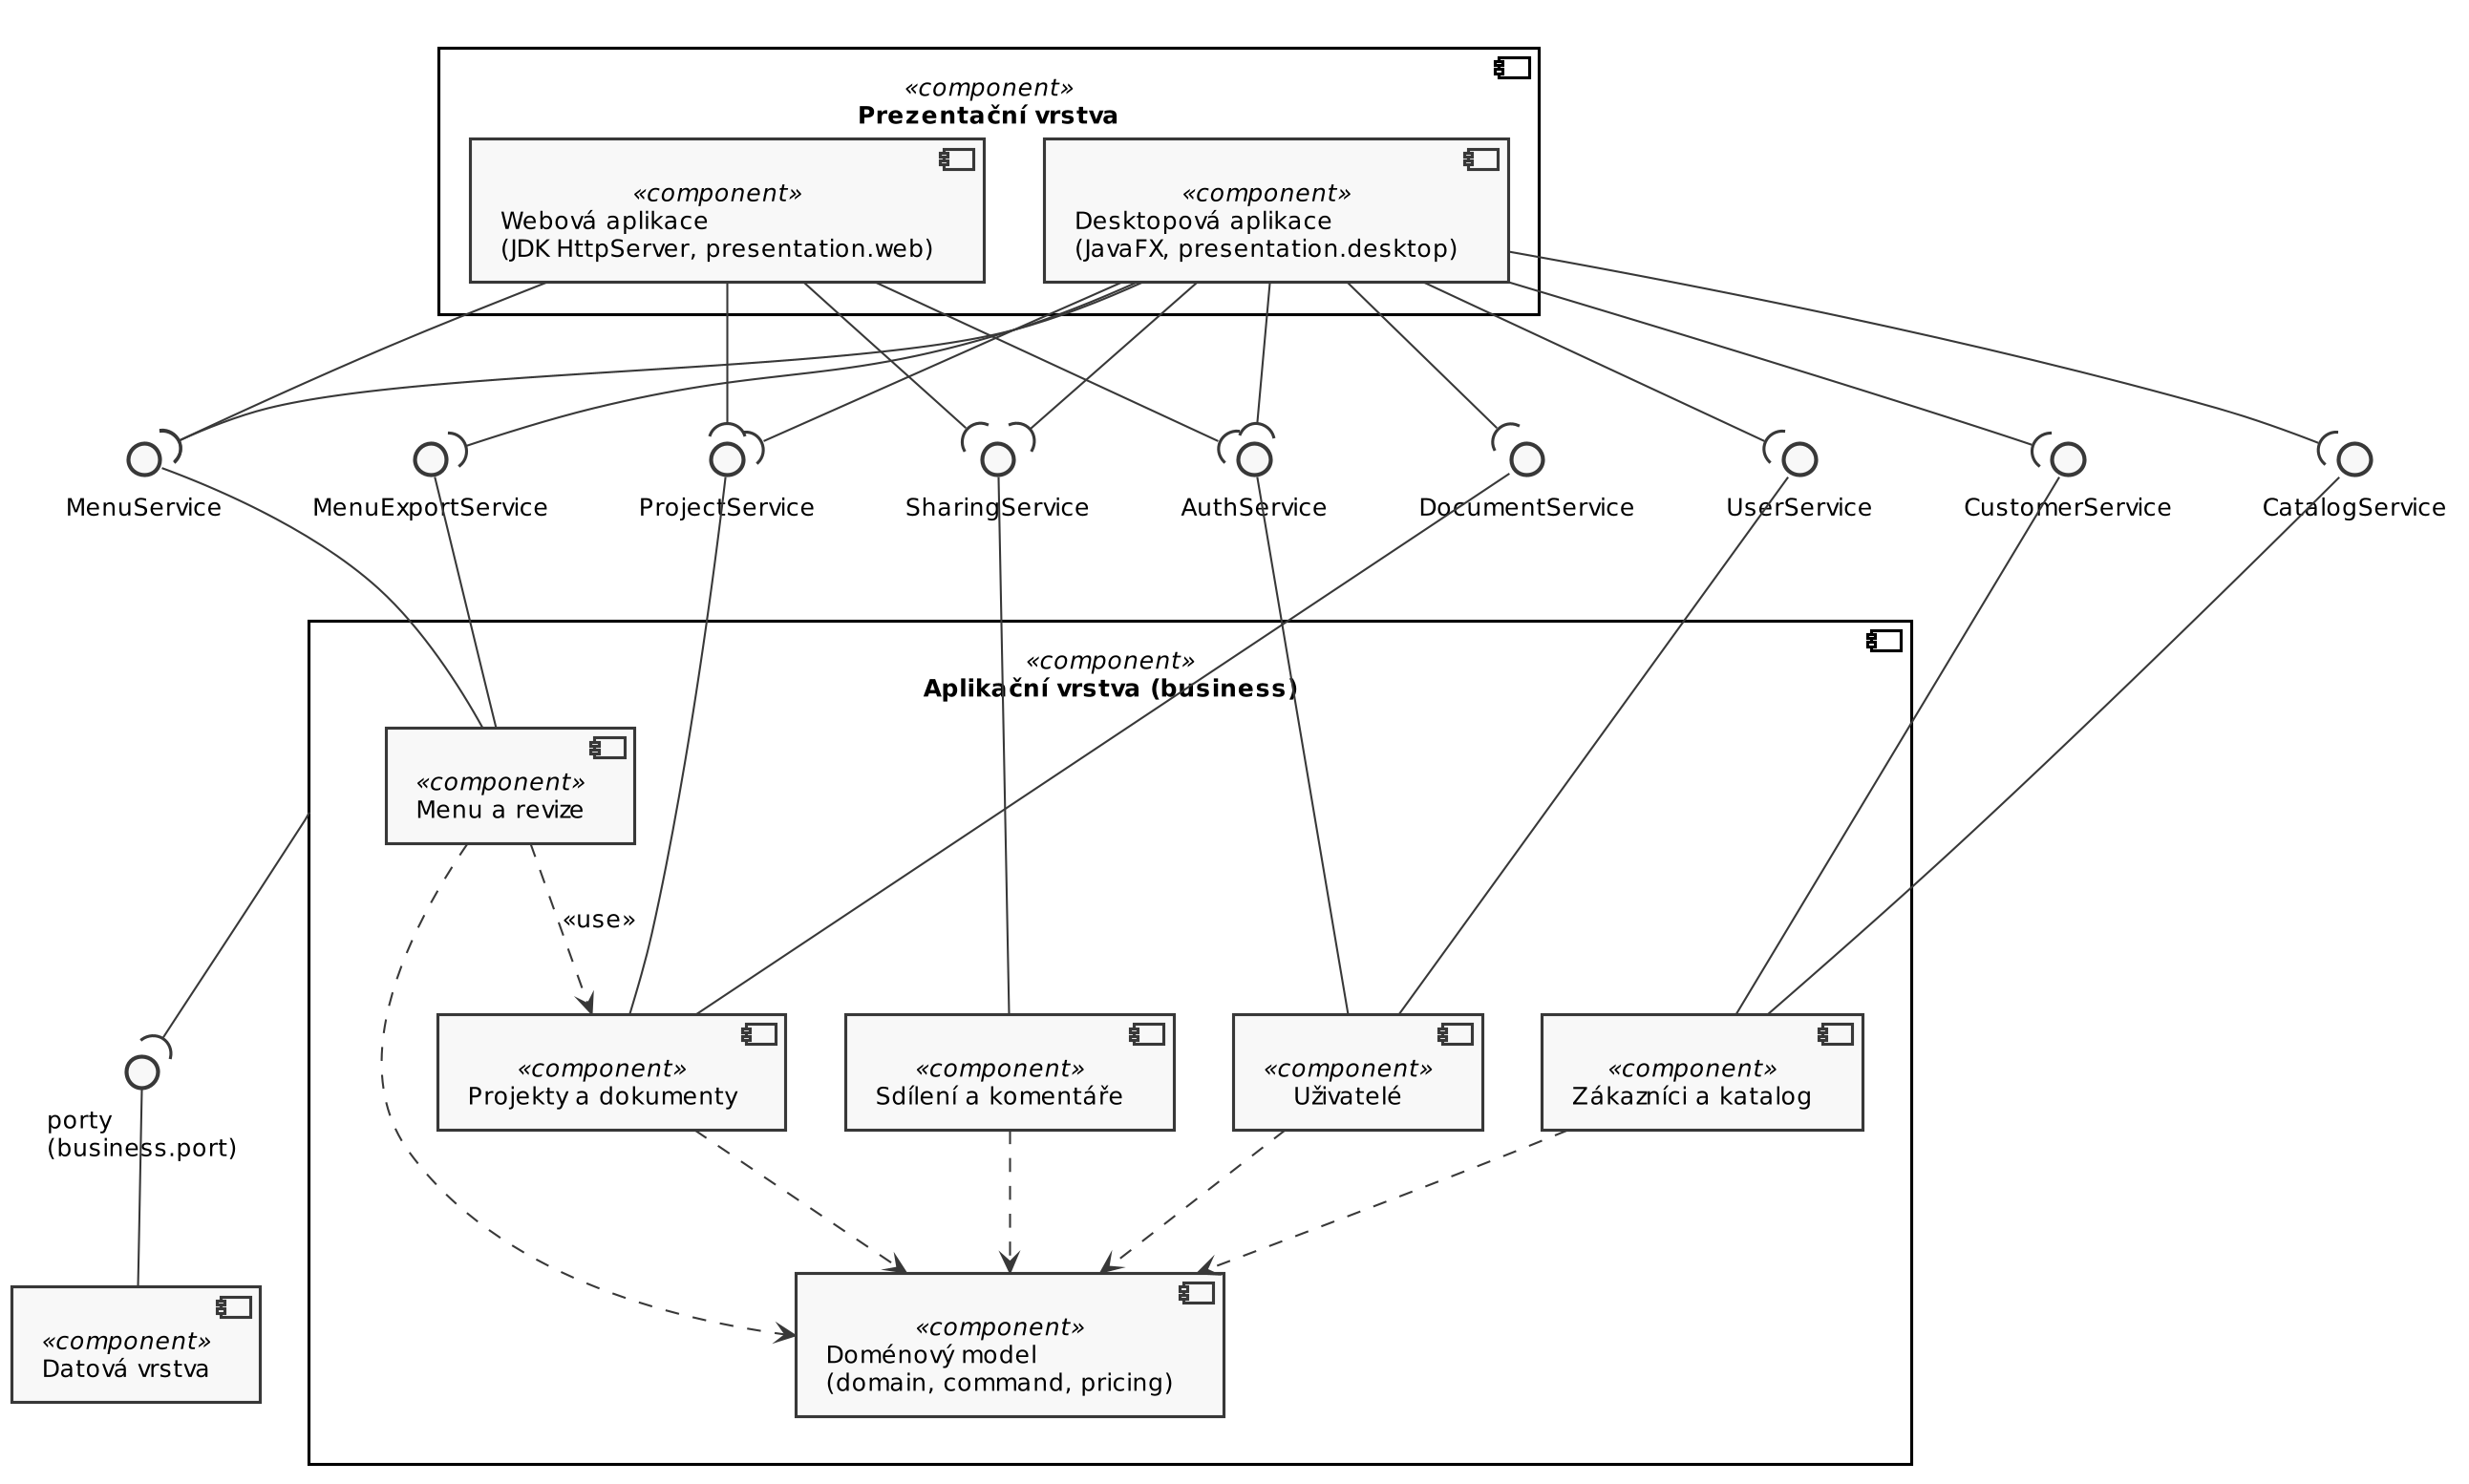
\includegraphics[width=0.85\textheight,height=\textwidth,keepaspectratio,angle=90]{component.png}
  \caption{Diagram komponent -- prezentační a aplikační vrstva}
  \label{fig:komponenty}
\end{figure}
\clearpage

\subsubsection*{Prezentační vrstva}

\begin{description}[itemsep=2pt,style=unboxed]
  \item[Desktopová aplikace] balíček \texttt{presentation.desktop}. Obsahuje okna a dialogy v JavaFX (\texttt{MainWindow}, \texttt{MenuEditorWindow}, \texttt{CommentsWindow}, \texttt{CompareRevisionsWindow}, \texttt{UsersWindow}, \texttt{CustomersWindow}, \texttt{CatalogWindow}, \texttt{ShareDialog} a další). Vstupní třída je \texttt{DesktopApp}. Desktopová aplikace pokrývá práci pracovníka a administrátora, a proto používá všech devět aplikačních služeb.
  \item[Webová aplikace] balíček \texttt{presentation.web}. Třída \texttt{WebServer} spouští \texttt{HttpServer} z JDK a registruje dva obslužné objekty. \texttt{MenuHandler} obsluhuje stránky zákazníka se sdílenou nabídkou a komentáři (\ucref{11}, \ucref{12}) a stránku prošlého odkazu. \texttt{ManagerHandler} obsluhuje přihlášení manažera a přehled projektů pouze pro čtení (\ucref{15}). Manažer vidí jen projekty pracovníků, kteří mu podléhají. Relace si pamatuje pouze identifikátor uživatele a při každém požadavku uživatele znovu načte, takže deaktivovaný manažer nebo manažer bez role ztratí přístup okamžitě. Po pěti chybných přihlášeních během deseti minut server další pokusy odmítne. Odpovědi nesou bezpečnostní hlavičky (Content-Security-Policy, nosniff, no-referrer) a cookie relace má za HTTPS příznak \texttt{Secure}. Server ukončí požadavek, který trvá déle než 30 sekund. HTML stránky skládají třídy \texttt{MenuPage} a \texttt{ManagerPage}. \texttt{ExpiredLinkScheduler} jednou denně zneplatní prošlé odkazy (\ucref{18}). Samostatný webový režim spouští třída \texttt{WebMain}. Webová aplikace používá služby \texttt{AuthService}, \texttt{ProjectService}, \texttt{MenuService} a \texttt{SharingService}.
\end{description}

\subsubsection*{Aplikační vrstva}

Aplikační vrstva je rozdělena na vnitřní komponenty podle oblastí. Každá oblast poskytuje své služby jako rozhraní pro prezentační vrstvu (vzor Facade). Služby jsou v balíčku \texttt{business.service}.

\begin{description}[itemsep=2pt,style=unboxed]
  \item[Uživatelé] \texttt{AuthService} (přihlášení) a \texttt{UserService} (správa uživatelů a rolí, \ucref{16}). Pravidla rolí jsou na jednom místě ve třídě \texttt{AccessPolicy} z doménového modelu. Role se sčítají. Pracovník používá desktopovou aplikaci, administrátor administrátorský režim a manažer webový přehled.
  \item[Zákazníci a katalog] \texttt{CustomerService} (evidence zákazníků) a \texttt{CatalogService} (katalog produktů a alergenů).
  \item[Projekty a dokumenty] \texttt{ProjectService} (projekty a jejich strom obsahu) a \texttt{DocumentService} (složky a dokumenty v úložišti).
  \item[Menu a revize] \texttt{MenuService} (menu, revize, editor menu a porovnání revizí) a \texttt{MenuExportService} (export revize do PDF, \ucref{14}). \texttt{MenuExportService} uloží vytvořený soubor přes \texttt{DocumentService}, proto komponenta závisí na komponentě Projekty a dokumenty.
  \item[Sdílení a komentáře] \texttt{SharingService} (sdílení revize odkazem, komentáře zákazníka, jejich vyřízení a zneplatnění prošlých odkazů).
  \item[Doménový model] balíčky \texttt{business.domain} (doménové třídy, například \texttt{Project}, \texttt{MenuRevision}, \texttt{Folder}), \texttt{business.command} (příkazy editoru menu a \texttt{MenuEditor}) a \texttt{business.pricing} (strategie výpočtu ceny \texttt{PriceStrategy}). Pravidla domény jsou zde a služby je pouze volají. Podrobný popis tříd je v \odkaz{sec:a5}{návrhu doménového modelu}.
\end{description}

\clearpage
\begin{figure}[H]
  \centering
  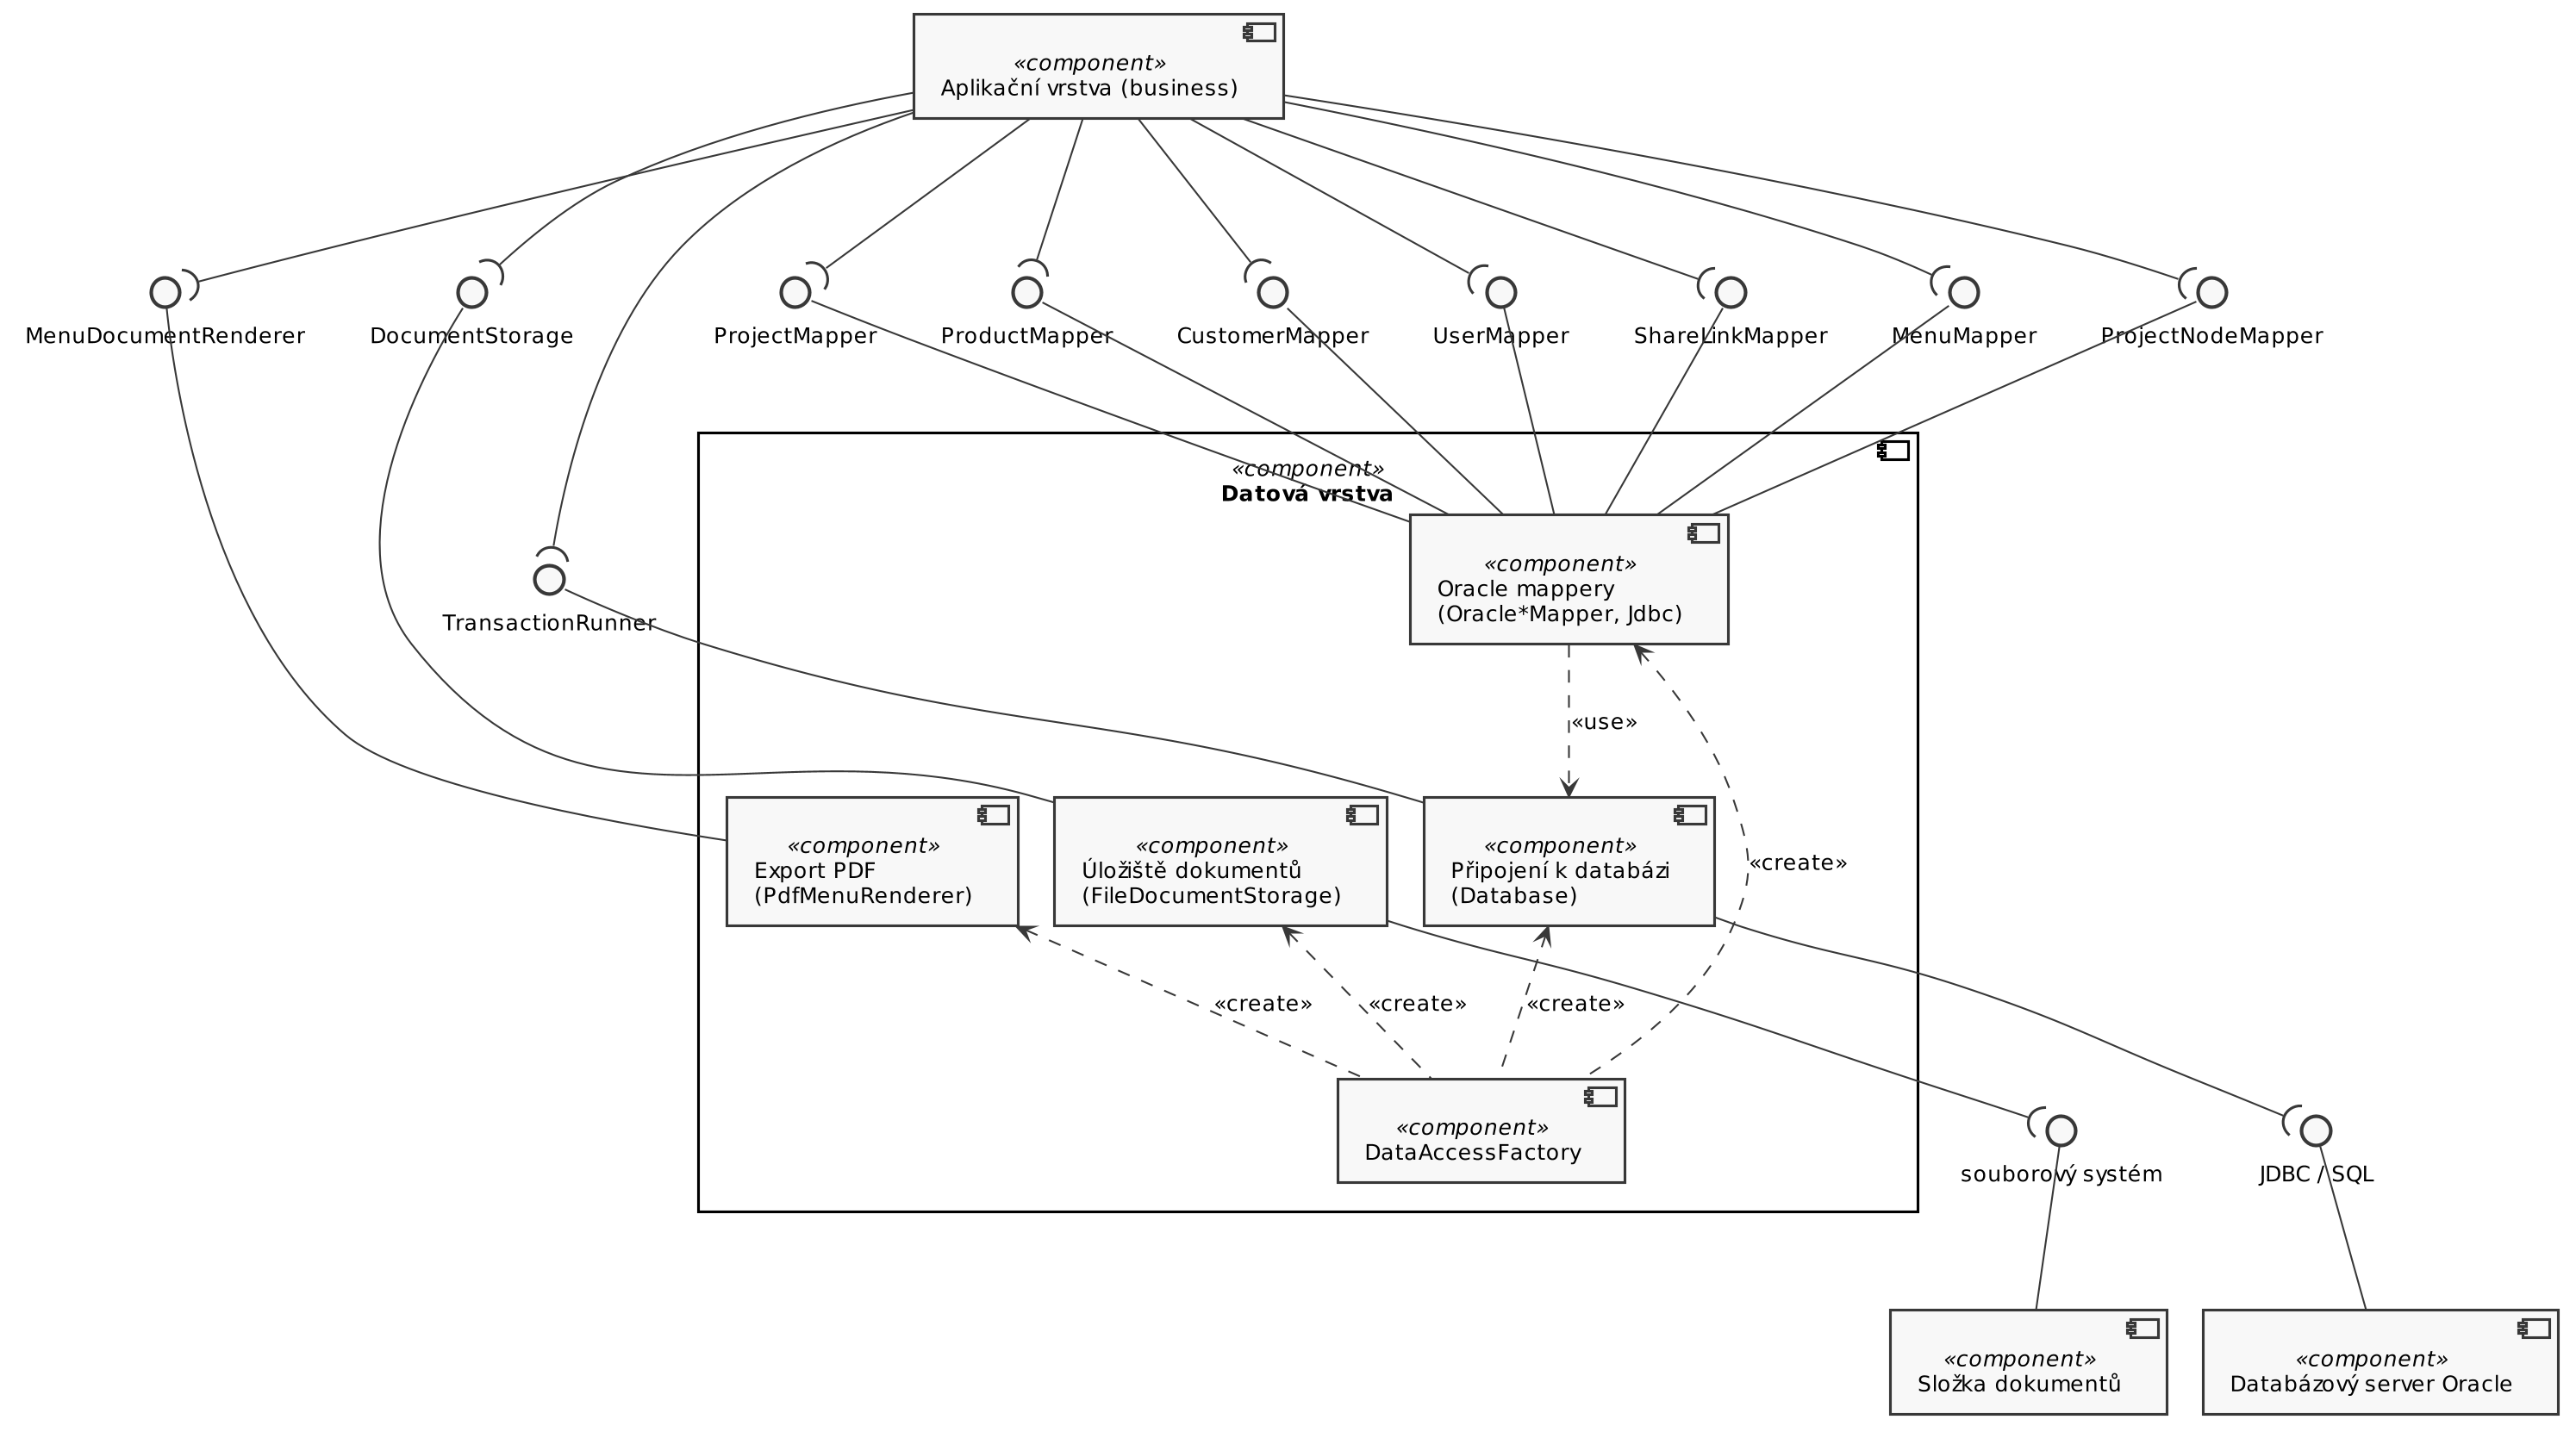
\includegraphics[width=0.85\textheight,height=\textwidth,keepaspectratio,angle=90]{component-data.png}
  \caption{Diagram komponent -- porty aplikační vrstvy a datová vrstva}
  \label{fig:komponenty-data}
\end{figure}
\clearpage

\subsubsection*{Porty aplikační vrstvy}

Aplikační vrstva sama definuje rozhraní, která potřebuje od datové vrstvy. Rozhraní jsou v balíčku \texttt{business.port}. Tabulka~\ref{tab:porty} uvádí, které služby které rozhraní vyžadují (podle konstruktorů služeb) a která třída datové vrstvy je implementuje.

\begin{table}[H]
\centering
\small
\begin{tabularx}{\textwidth}{ll>{\raggedright\arraybackslash}X}
\toprule
\textbf{Rozhraní} & \textbf{Implementace} & \textbf{Vyžadují služby} \\
\midrule
\texttt{UserMapper} & \texttt{OracleUserMapper} & \texttt{AuthService}, \texttt{UserService} \\
\texttt{CustomerMapper} & \texttt{OracleCustomerMapper} & \texttt{CustomerService}, \texttt{ProjectService} \\
\texttt{ProductMapper} & \texttt{OracleProductMapper} & \texttt{CatalogService}, \texttt{MenuService} \\
\texttt{ProjectMapper} & \texttt{OracleProjectMapper} & \texttt{ProjectService}, \texttt{DocumentService}, \texttt{MenuService}, \texttt{SharingService} \\
\texttt{ProjectNodeMapper} & \texttt{OracleProjectNodeMapper} & \texttt{ProjectService}, \texttt{DocumentService}, \texttt{MenuService} \\
\texttt{MenuMapper} & \texttt{OracleMenuMapper} & \texttt{MenuService}, \texttt{SharingService} \\
\texttt{ShareLinkMapper} & \texttt{OracleShareLinkMapper} & \texttt{SharingService} \\
\texttt{TransactionRunner} & \texttt{Database} & všechny služby kromě \texttt{MenuExportService} \\
\texttt{DocumentStorage} & \texttt{FileDocumentStorage} & \texttt{DocumentService} \\
\texttt{MenuDocumentRenderer} & \texttt{PdfMenuRenderer} & \texttt{MenuExportService} \\
\bottomrule
\end{tabularx}
\caption{Porty aplikační vrstvy a jejich implementace}
\label{tab:porty}
\end{table}

\subsubsection*{Datová vrstva a externí systémy}

\begin{description}[itemsep=2pt,style=unboxed]
  \item[Oracle mappery] balíček \texttt{data.oracle}. Třídy \texttt{Oracle*Mapper} implementují rozhraní mapperů (vzor Data Mapper) a převádějí doménové objekty na řádky tabulek a zpět. Společné volání JDBC (dotaz, vložení s vrácením identifikátoru, úprava) je v pomocné třídě \texttt{Jdbc}.
  \item[Připojení k databázi] třída \texttt{Database} je jediná instance (Singleton), která otevírá připojení JDBC pro každou transakci a drží je pro aktuální vlákno. Implementuje \texttt{TransactionRunner}, takže služba spustí práci v transakci a \texttt{Database} provede commit nebo rollback. Mappery získávají připojení přes \texttt{Jdbc} z této instance.
  \item[Úložiště dokumentů] \texttt{FileDocumentStorage} (balíček \texttt{data.file}) ukládá soubory dokumentů do složky nastavené klíčem \texttt{documents.dir}. Pro testy existuje také \texttt{InMemoryDocumentStorage}.
  \item[Export PDF] \texttt{PdfMenuRenderer} vytváří z revize menu dokument PDF pomocí knihovny Apache PDFBox.
  \item[DataAccessFactory] továrna, která podle konfigurace vytvoří \texttt{Database} a všechny implementace portů. Zbytek aplikace zná jen rozhraní z \texttt{business.port}.
  \item[Databázový server Oracle] externí komponenta, ke které se \texttt{Database} připojuje přes rozhraní JDBC a jazyk SQL. Obsahuje schéma \texttt{CATERING}.
  \item[Složka dokumentů] adresář v souborovém systému, do kterého \texttt{FileDocumentStorage} zapisuje soubory.
\end{description}

\subsubsection*{Pravidlo závislostí a důvody rozdělení}

Závislosti vedou z prezentační vrstvy do aplikační vrstvy. Datová vrstva závisí také na aplikační vrstvě, protože implementuje její rozhraní (prezentace $\rightarrow$ aplikační vrstva $\leftarrow$ data). Aplikační vrstva neimportuje žádnou třídu z balíčků \texttt{presentation} ani \texttt{data}. Konkrétní implementace jí předá až \texttt{AppContext} v konstruktorech služeb.

Toto rozdělení má tři důvody. Doménová pravidla jsou na jednom místě a nezávisí na databázi ani na uživatelském rozhraní, takže je lze testovat bez databáze (testy používají vlastní implementace portů a \texttt{InMemoryDocumentStorage}). Úložiště lze vyměnit bez zásahu do služeb, protože služby znají jen rozhraní. Desktopová i webová aplikace volají stejné služby, takže pravidla se nepíší dvakrát. Například sdílenou nabídku zobrazuje zákazníkovi webová stránka přes \texttt{SharingService} a pracovník vyřizuje komentáře ve stejné službě z desktopové aplikace.

\subsection{Diagram nasazení}\label{sec:arch:nasazeni}

Diagram na obrázku~\ref{fig:nasazeni-a6} ukazuje skutečné nasazení ve společnosti. Navazuje na \odkaz{sec:tech}{první představu o nasazení}. Proti ní je upřesněn spustitelný artefakt a webové rozhraní. Aplikace naslouchá na portu 8080 a protokol HTTPS na portu 443 zajišťuje reverzní proxy na aplikačním serveru.

\clearpage
\begin{figure}[H]
  \centering
  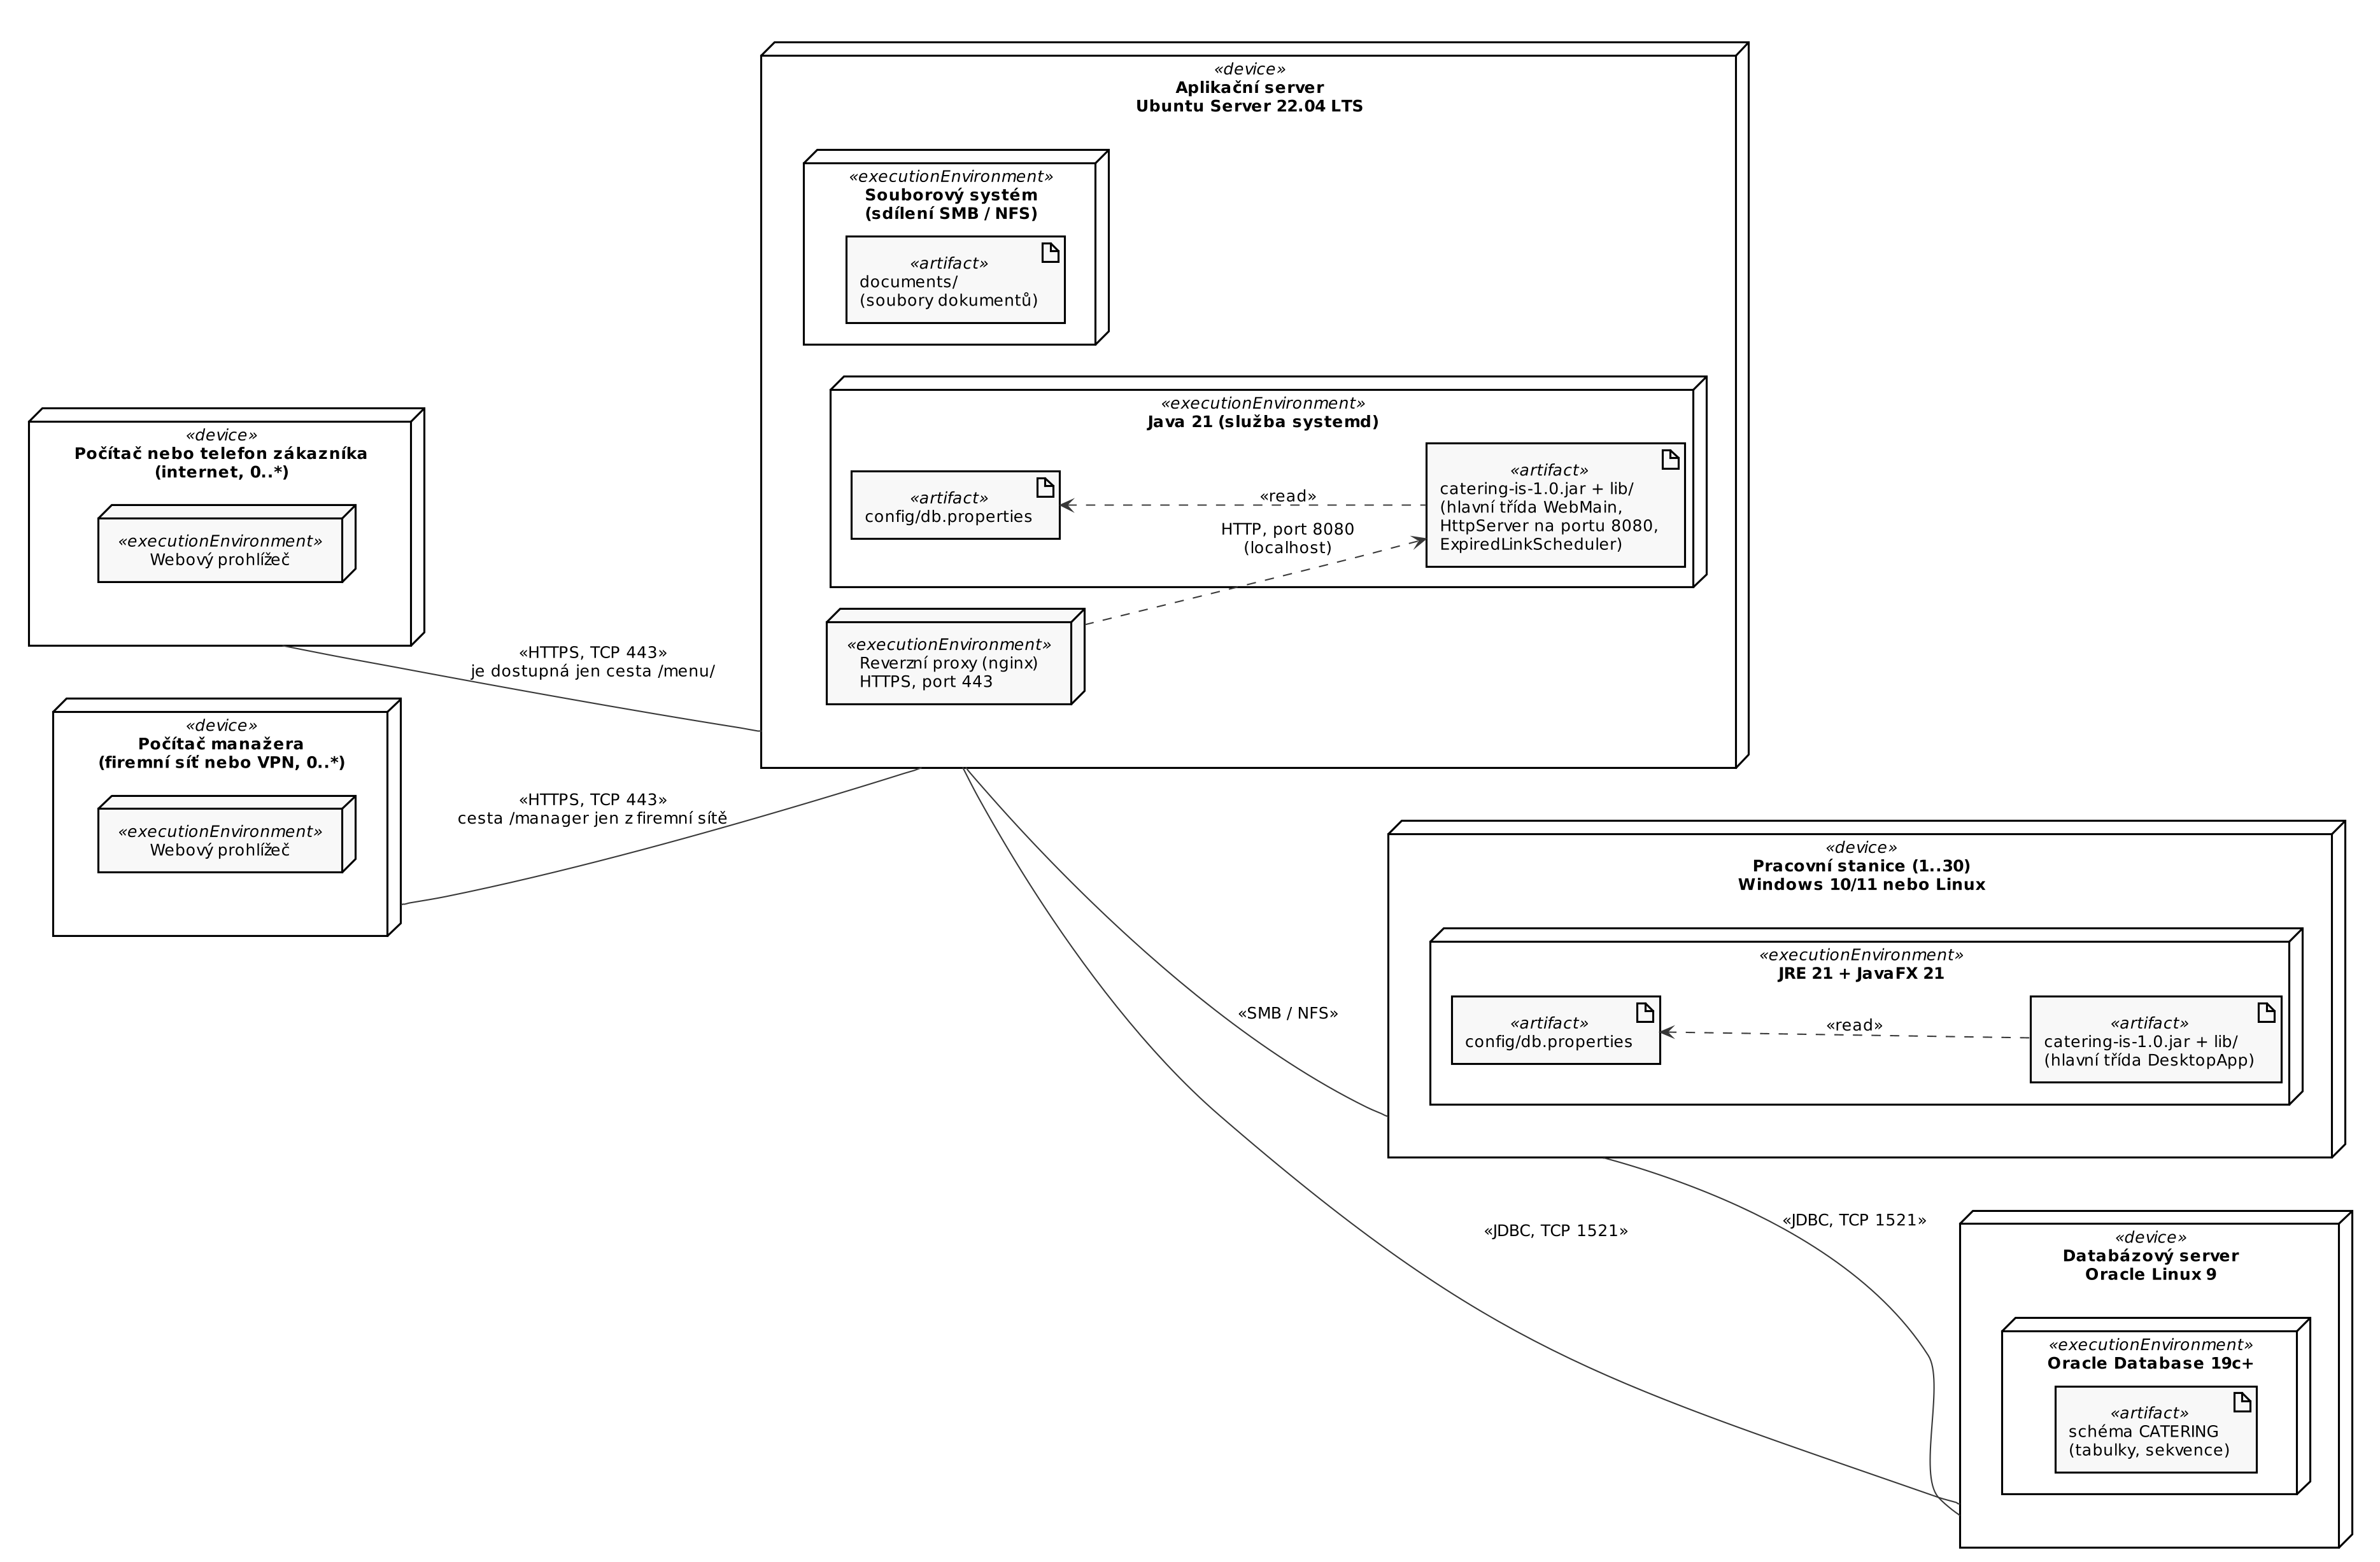
\includegraphics[width=0.85\textheight,height=\textwidth,keepaspectratio,angle=90]{deployment-a6.png}
  \caption{Diagram nasazení}
  \label{fig:nasazeni-a6}
\end{figure}
\clearpage

\begin{description}[itemsep=2pt,style=unboxed]
  \item[Pracovní stanice (1 až 30)] Windows 10/11 nebo Linux s prostředím Java~21 a JavaFX~21. Běží zde desktopová aplikace (\texttt{catering-is-1.0.jar} s knihovnami ve složce \texttt{lib/}, hlavní třída \texttt{DesktopApp}) se souborem \texttt{config/db.properties}. Stanice se připojuje přes JDBC k databázovému serveru a čte a zapisuje soubory ve sdílené složce dokumentů na aplikačním serveru (SMB nebo NFS).
  \item[Aplikační server] Ubuntu Server 22.04 LTS s Javou~21. Stejný artefakt běží jako služba systemd ve webovém režimu (hlavní třída \texttt{WebMain}). Obsahuje \texttt{HttpServer} na portu 8080 a \texttt{ExpiredLinkScheduler}. Před aplikací je reverzní proxy nginx, která přijímá HTTPS na portu 443. Z internetu předává na \texttt{localhost:8080} pouze cesty \texttt{/menu/} pro zákazníky. Přehled manažera \texttt{/manager} je dostupný jen z firemní sítě nebo přes VPN. Server také sdílí složku \texttt{documents/} pracovním stanicím.
  \item[Databázový server] Oracle Linux 9 s Oracle Database 19c nebo novější. Schéma \texttt{CATERING} s tabulkami a sekvencemi. Spojení JDBC přijímá na portu 1521.
  \item[Klientský počítač nebo telefon] zákazník a manažer používají jen webový prohlížeč a k aplikačnímu serveru přistupují přes HTTPS.
\end{description}

\subsection{Instalace a spuštění}\label{sec:arch:instalace}

\begin{enumerate}[itemsep=2pt]
  \item \textbf{Databázový server.} Nainstalovat Oracle Database, vytvořit uživatele (schéma) \texttt{CATERING} a spustit ze složky \texttt{db} skripty databáze, nejprve \texttt{01\_schema.sql} a potom \texttt{02\_seed.sql}. Vytvoří tabulky, sekvence a výchozí data. Povolit port 1521 pro aplikační server a pracovní stanice.
  \item \textbf{Sestavení.} Na počítači s JDK~21 a Maven ve složce \texttt{app} spustit:
\begin{verbatim}
mvn package
mvn dependency:copy-dependencies -DincludeScope=runtime \
    -DoutputDirectory=target/lib
\end{verbatim}
Vznikne \texttt{target/catering-is-1.0.jar} a složka \texttt{target/lib} s knihovnami (JavaFX, ovladač Oracle JDBC, PDFBox, ZXing).
  \item \textbf{Konfigurace.} Vedle artefaktu vytvořit soubor \texttt{config/db.properties} podle vzoru \texttt{db.properties.example} ze stejné složky. Klíče jsou \texttt{db.url} (například \texttt{jdbc:oracle:thin:@//dbserver:1521/služba}), \texttt{db.user}, \texttt{db.password}, \texttt{documents.dir} (na serveru místní cesta ke složce dokumentů, na stanici cesta k připojené sdílené složce), \texttt{web.port} (výchozí 8080), \texttt{web.embedded} (výchozí \texttt{false}, viz níže) a \texttt{web.baseUrl} (veřejná adresa webu, ze které se skládají odkazy pro zákazníky, například \texttt{https://catering.firma.cz}). Aplikace hledá soubor relativně k pracovní složce, proto se spouští ze složky, která obsahuje \texttt{config/}. Jiné umístění souboru lze zadat parametrem \texttt{-Dcatering.config=cesta}.
  \item \textbf{Aplikační server.} Nainstalovat Javu~21, nakopírovat artefakt, \texttt{lib/} a \texttt{config/}. Jako službu systemd spustit:
\begin{verbatim}
java -cp "catering-is-1.0.jar:lib/*" \
     cz.vsb.catering.presentation.web.WebMain
\end{verbatim}
Nastavit reverzní proxy s certifikátem na port 443 a sdílet složku dokumentů přes SMB nebo NFS.
  \item \textbf{Pracovní stanice.} Nainstalovat Javu~21, nakopírovat artefakt, \texttt{lib/} a \texttt{config/} a připojit sdílenou složku dokumentů. Aplikaci spustit příkazem:
\begin{verbatim}
java --module-path lib --add-modules javafx.controls \
     -cp "catering-is-1.0.jar:lib/*" \
     cz.vsb.catering.presentation.desktop.DesktopApp
\end{verbatim}
Ve Windows se v cestě tříd místo dvojtečky píše středník a příkaz se zapíše na jeden řádek.
\end{enumerate}

Webový server a denní zneplatnění odkazů běží jen na aplikačním serveru (\texttt{WebMain}). Desktopová aplikace je spustí také, pouze pokud je v konfiguraci \texttt{web.embedded=true}. To se používá jen při vývoji a předvedení na jednom počítači. Na pracovních stanicích zůstává výchozí hodnota \texttt{false}.

\textbf{Vývojová varianta.} Při vývoji a předvedení běží vše na jednom počítači. Databáze Oracle běží v kontejneru Docker na portu 1521, \texttt{documents.dir} je místní složka \texttt{./documents} a konfigurace obsahuje \texttt{web.embedded=true} a aplikace se spouští ze složky \texttt{app} příkazem \texttt{mvn javafx:run} (desktop i web na portu 8080) nebo \texttt{mvn exec:java} (pouze webový režim \texttt{WebMain}). Webové stránky lze otevřít i z jiného počítače v síti na adrese \texttt{http://počítač:8080}.
\endgroup
